%%%%%%%%%%%%%%%%%%%%%%%%%%%%%%%%%%%%%%%%%
% Beamer Presentation
% LaTeX Template
% Version 1.0 (10/11/12)
%
% This template has been downloaded from:
% http://www.LaTeXTemplates.com
%
% License:
% CC BY-NC-SA 3.0 (http://creativecommons.org/licenses/by-nc-sa/3.0/)
%
%%%%%%%%%%%%%%%%%%%%%%%%%%%%%%%%%%%%%%%%%

%----------------------------------------------------------------------------------------
%	PACKAGES AND THEMES
%----------------------------------------------------------------------------------------

\documentclass{beamer}
\mode<presentation> {
\usetheme{Madrid}
}
\usepackage{url}
\usepackage{lmodern}
\usepackage{graphicx}
\usepackage{booktabs}

% for mathematics
\usepackage{amsmath}
\usepackage{amsthm}

%----------------------------------------------------------------------------------------
%	TITLE PAGE
%----------------------------------------------------------------------------------------

\title[Financial mathematics with Python]{UROPS Project Presentation 2} % The short title appears at the bottom of every slide, the full title is only on the title page

\author{Wang Zexin} % Your name
\institute[NUS]
{
Chpter 11 Statistics\\
of Python for Finance\\[3mm]
Variance Reduction Techniques\\
of Monte Carlo methods in Financial Engineering\\[3mm]
\medskip
\textit{Quantitative Finance\\
National University of Singapore\\}
}
\date{\today}

\begin{document}
%----------------------------------------------------------------------------------------
%	TITLE PAGE
%----------------------------------------------------------------------------------------
\begin{frame}
\titlepage
\end{frame}

%----------------------------------------------------------------------------------------
%	TABLE OF CONTENTS
%----------------------------------------------------------------------------------------

%------------------------------------------------
\begin{frame}
\frametitle{Today's Agenda}
\tableofcontents
\end{frame}

%------------------------------------------------
\begin{frame}
\frametitle{Changes due to different Python version}
We are using Python 3.6 while the version in the book is Python 2.7\\
So here is a list of items to change\\[2mm]
\begin{itemize}
	\item print x now becomes print(x)
	\item dict.iteritems() now becomes dict.items()
	\item xrange now becomes range
	\item lambda (k, v) : (v, k) is no longer available
	\item instead we can only use: lambda x : (x[1], x[0])
	\item x / 2 is float division, while x // 2 is integer division
\end{itemize}
\end{frame}

%------------------------------------------------
\begin{frame}
\frametitle{Installation requirements - pandas\_datareader}
We are going to install pandas\_datareader instead of pandas.io.data\\[2mm]
Reason being that: ImportError: The pandas.io.data module is moved to a separate package (pandas-datareader). \\[2mm]
Also, Anaconda does not support direct installation of this new package.\\[5mm]
Hence, here is one line of code which you can type in Anaconda Prompt.\\[2mm]
conda install -c https://conda.anaconda.org/anaconda pandas-datareader\\
\end{frame}

%------------------------------------------------
\section{Statistics} %------------------------------------------------

%------------------------------------------------

\begin{frame}
\frametitle{Chapter 11 Statistics}
We shall go through these useful methods\\[4mm]
\begin{itemize}
	\item Normality test
	\item Portfolio theory
	\item Principal component analysis
	\item Bayesian Regression
\end{itemize}
\end{frame}

\subsection{Normality test}
%------------------------------------------------
\begin{frame}
\frametitle{Normality test - wrapper functions for np arrays}
\begin{figure}[H]
	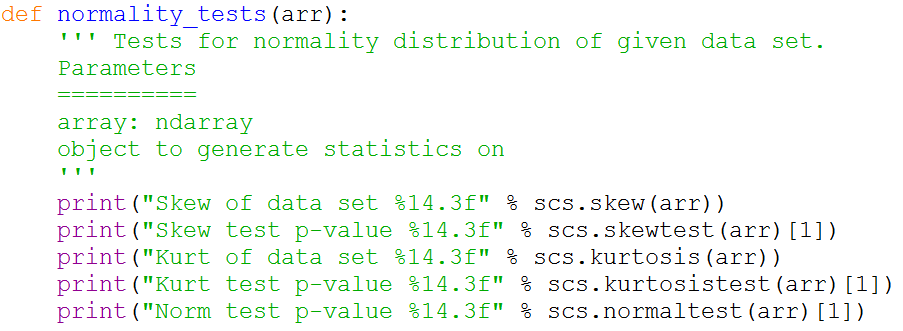
\includegraphics[scale=0.5]{normality_test.png}
\end{figure}
\end{frame}

\subsection{Portfolio Optimization}

%------------------------------------------------
\begin{frame}
\frametitle{Portfolio Optimization}
Assumptions we made are:
\begin{itemize}
	\item Stock prices follow CAPM mostly
	\item Use only close price of the stock (adj close)
	\item Use csv.reader instead of pandas in this section
\end{itemize}
\end{frame}

%------------------------------------------------
\begin{frame}
\frametitle{Portfolio Optimization}
We are going to optimize based on these:
\begin{itemize}
	\item higher order statistics function
	\item maximization of Sharpe ratio - MVE
	\item minimization of portfolio variance - MVP
	\item Efficient Frontier
	\item Capital Market Line
\end{itemize}
\end{frame}

%------------------------------------------------
\begin{frame}
\frametitle{Read stock data from CSV files}
\begin{figure}[H]
	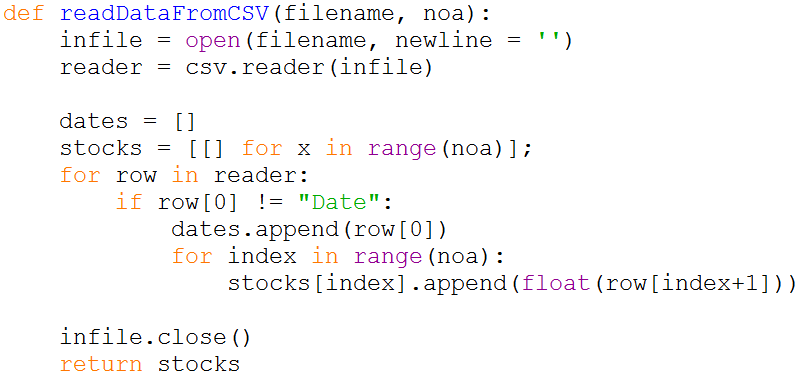
\includegraphics[scale=0.55]{readDataFromCsv.png}
\end{figure}
\end{frame}

%------------------------------------------------
\begin{frame}
\frametitle{Convert stock prices to returns}
There is a bug in the code provided in the book. \\
nparray.mean() will only calculate one average for the entire 2D array
\begin{figure}[H]
	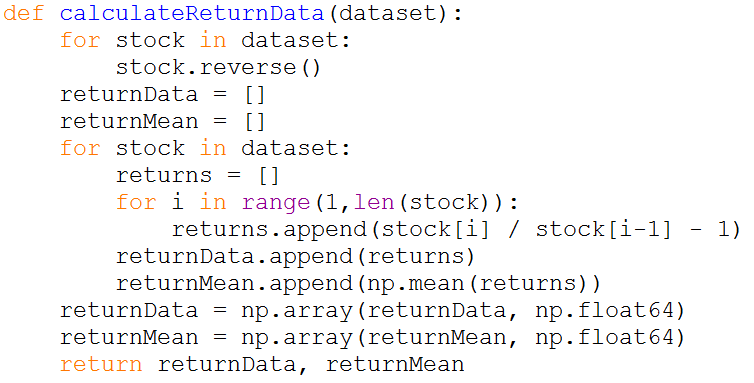
\includegraphics[scale=0.55]{calculate_return_data.png}
\end{figure}
\end{frame}

%------------------------------------------------
\begin{frame}
\frametitle{Generate statistics function}
We can create a high order function to generate statistics function\\
for a given set of return data
\begin{figure}[H]
	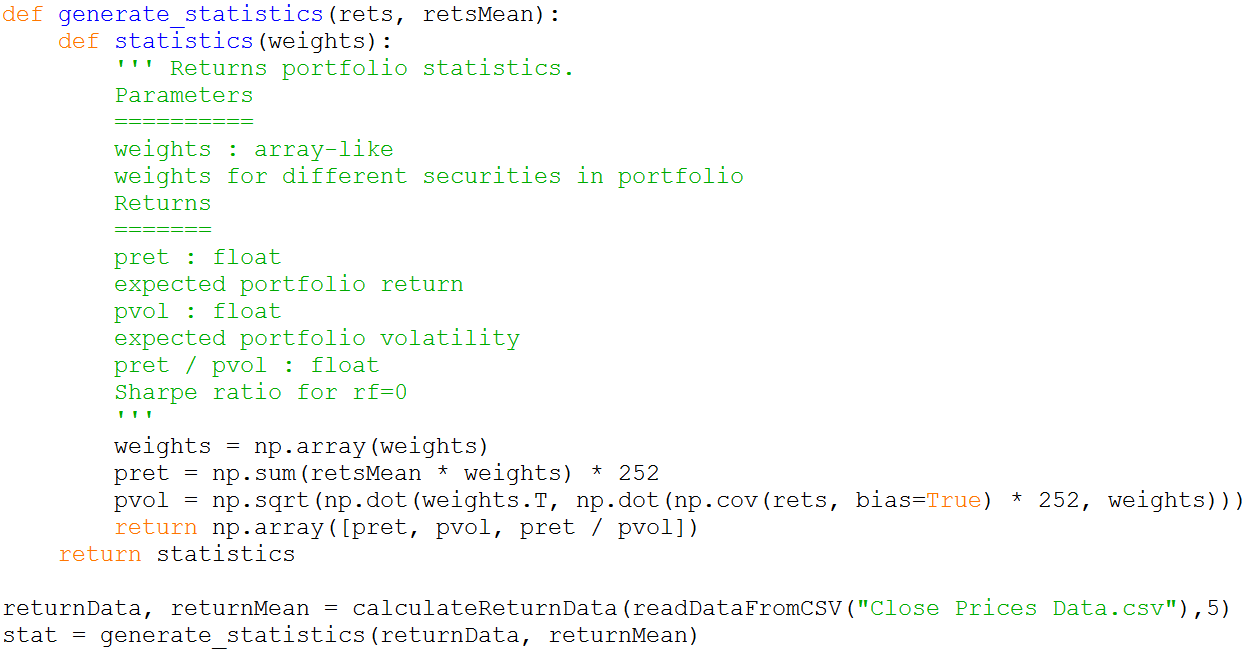
\includegraphics[scale=0.37]{generate_statistics.png}
\end{figure}
\end{frame}

%------------------------------------------------
\begin{frame}
\frametitle{Optimize portfolio to maximise Sharpe ratio}
Make use of a new library scipy.optimize\\
Maximsie Sharpe ratio by minimizing negative Sharpe ratio
\begin{figure}[H]
	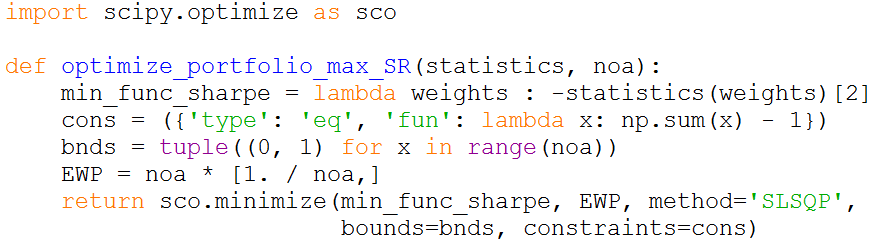
\includegraphics[scale=0.48]{optimize_max_SR.png}
\end{figure}
\begin{center}
Return value is a dictionary.\\
w = optimize\_portfolio\_max\_SR(stat, 5) \\
w['x'] is the optimal portfolio
\end{center}
\end{frame}

%------------------------------------------------
\begin{frame}
\frametitle{Optimize to minimise portfolio variance}
\begin{center}
Portfolio variance = $ w^{T} \Sigma w $
\end{center}
\begin{figure}[H]
	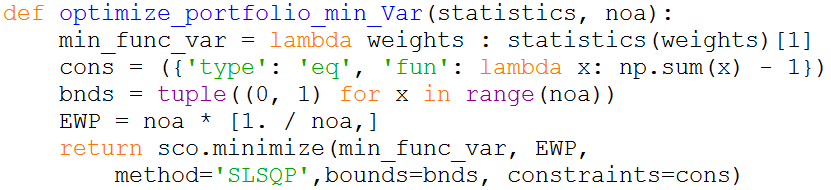
\includegraphics[scale=0.48]{optimize_min_Var.png}
\end{figure}
\begin{center}
Return value is a dictionary.\\
w = optimize\_portfolio\_min\_Var(stat, 5) \\
w['x'] is the optimal portfolio
\end{center}
\end{frame}

%------------------------------------------------
\begin{frame}
\frametitle{Generate Efficient Frontier}
We can set certain level of return to generate points on frontier.
\begin{figure}[H]
	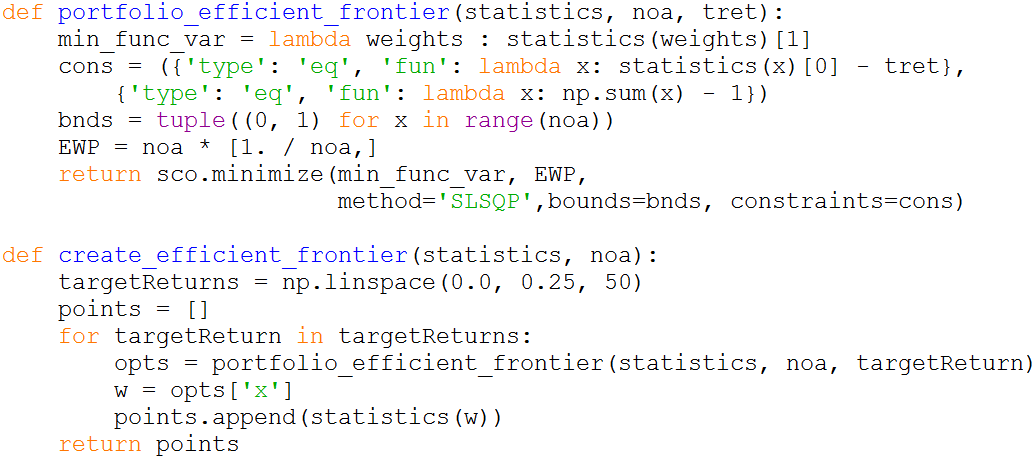
\includegraphics[scale=0.44]{generate_efficient_frontier.png}
\end{figure}
\end{frame}

%------------------------------------------------
\begin{frame}
\frametitle{Capital Market Line}
We can solve a system of equations to obtain this line.
\begin{center}
		$ a = r_{f} $\\
		$ a + bx = f(x) $\\
		$ b = f^{\prime}(x) $
\end{center}
\begin{figure}[H]
	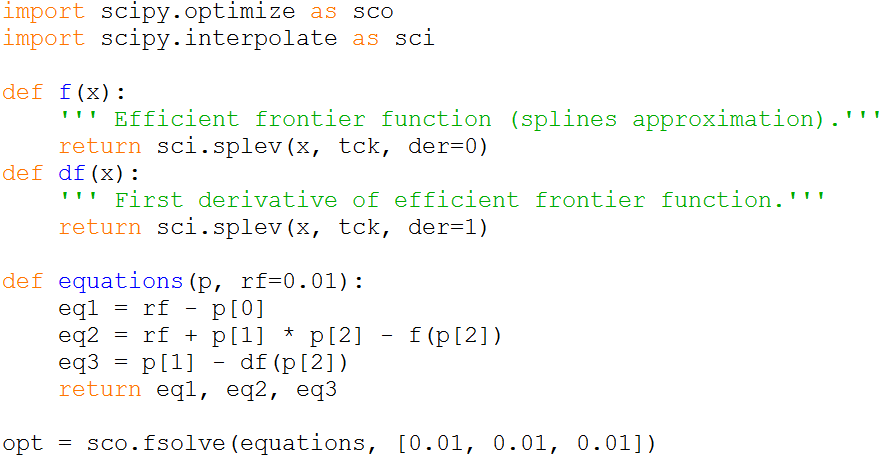
\includegraphics[scale=0.44]{generate_CML.png}
\end{figure}
\end{frame}

\subsection{Principal Componenet Analysis}

%------------------------------------------------
\begin{frame}
\frametitle{Principal Componenet Analysis}
\begin{itemize}
	\item Obtain data using pandas (initialization)
	\item Determine minimum number of components
	\item Create PCA Index
\end{itemize}
\end{frame}

%------------------------------------------------
\begin{frame}
\frametitle{PCA - initialization}
\begin{figure}[H]
	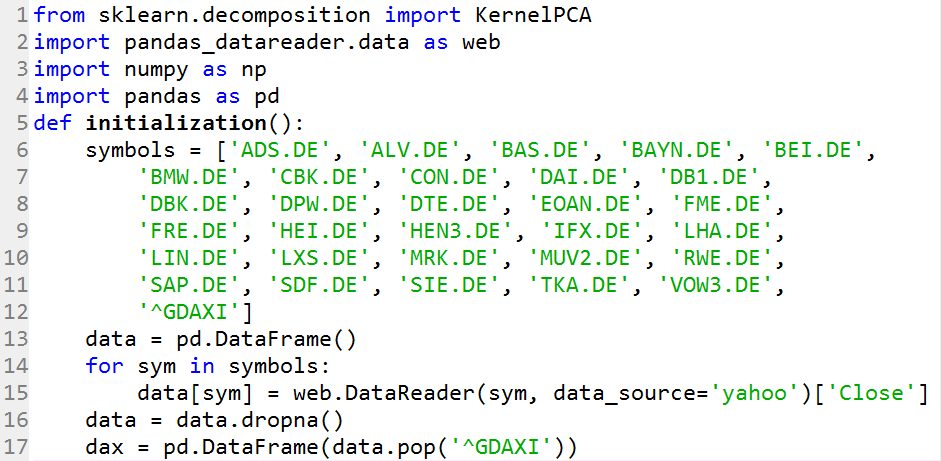
\includegraphics[scale=0.47]{pca_initialization.png}
\end{figure}
\end{frame}

%------------------------------------------------
\begin{frame}
\frametitle{PCA - Obtain stock data}
\begin{figure}[H]
	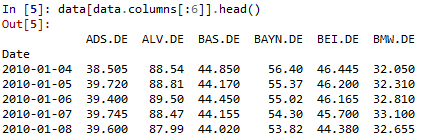
\includegraphics[scale=0.9]{PCA_retrieve_stock_data.png}
\end{figure}
\end{frame}

%------------------------------------------------
\begin{frame}
\frametitle{PCA - Determine number of components required}
\begin{figure}[H]
	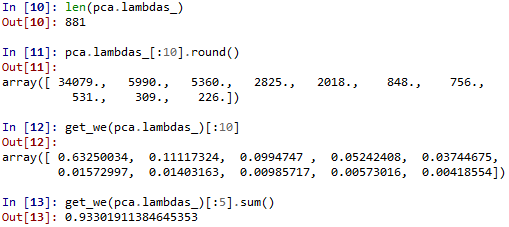
\includegraphics[scale=0.9]{PCA_first_five_components.png}
\end{figure}
More then 93.3\% of the variation is explained by the first five components!
\end{frame}

%------------------------------------------------
\begin{frame}
\frametitle{PCA - create index}
\begin{figure}[H]
	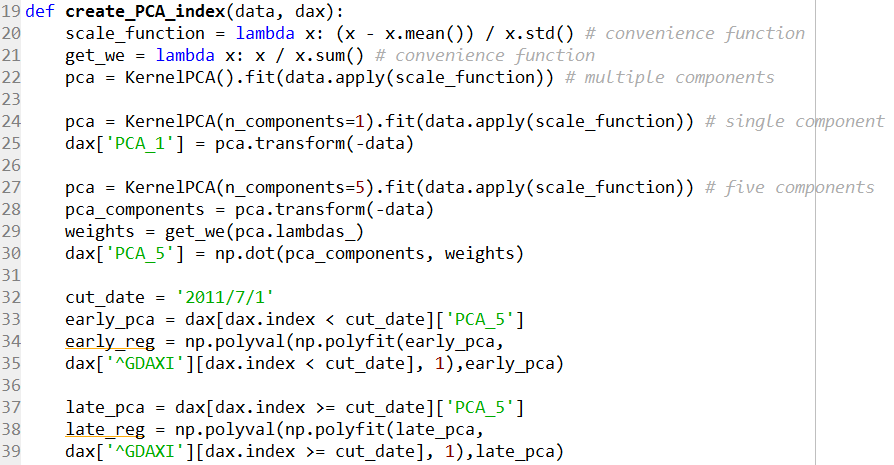
\includegraphics[scale=0.47]{create_PCA_index.png}
\end{figure}
\end{frame}

\subsection{Bayesian Regression}
%------------------------------------------------
\begin{frame}
\frametitle{Bayesian Regression}
\begin{itemize}
	\item Trouble shooting for package Pymc3
	\item Building of model
	\item Gaussian random walk
	\item Uniform model
	\item Optimization
\end{itemize}
\end{frame}

%------------------------------------------------
\begin{frame}
\frametitle{Trouble shooting for package Pymc3}
If this ValueError happens, go to the file font\_manager.py
\begin{figure}[H]
	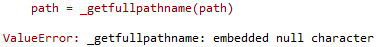
\includegraphics[scale=0.7]{pymc_error_1.png}
\end{figure}
and add in one line of code in the function win32InstalledFonts
\begin{figure}[H]
	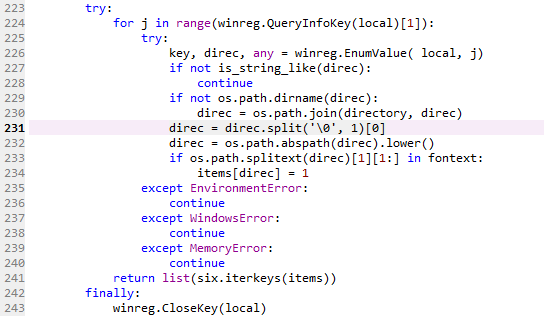
\includegraphics[scale=0.65]{pymc_error_2.png}
\end{figure}
\end{frame}

%------------------------------------------------
\begin{frame}
\frametitle{Building model}
If you can run this without having AttributeError,
\begin{figure}[H]
	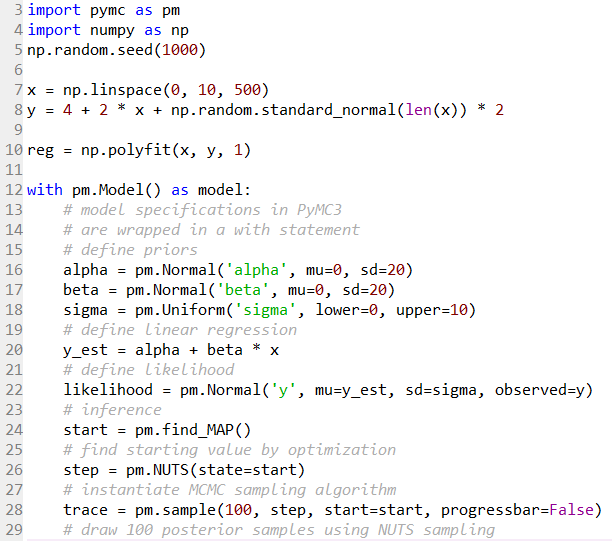
\includegraphics[scale=0.43]{bayesian_building_model.png}
\end{figure}
that means your version of Pymc3 is correctly installed.
\end{frame}

%------------------------------------------------
\begin{frame}
\frametitle{Trouble shooting for package Pymc3}
If this AttributeError (\_\_exit\_\_) happens,
\begin{figure}[H]
	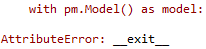
\includegraphics[scale=0.7]{pymc_error_3.png}
\end{figure}
that means you are using a version of Pymc3 in which with statement is not incorporated yet. You should go to Anaconda prompt and type:
conda install -c conda-forge pymc3
\end{frame}

%------------------------------------------------
\begin{frame}
\frametitle{Trouble shooting for package Pymc3}
If this AttributeError (TransformedVar) happens,
\begin{figure}[H]
	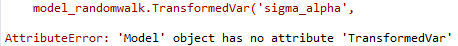
\includegraphics[scale=0.7]{pymc_error_4.png}
\end{figure}
when you are running the model below
\begin{figure}[H]
	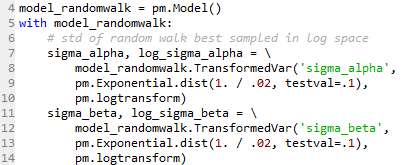
\includegraphics[scale=0.7]{bayesian_random_walk.png}
\end{figure}
the reason is that the attribute TransformedVar is removed from Pymc3.
\end{frame}

%------------------------------------------------
\begin{frame}
\frametitle{Trouble shooting for package Pymc3}
If the AttributeError (TransformVar) happens,
one fix is to use Exponential attribute of the package itself. \\ [4mm]
\begin{figure}[H]
	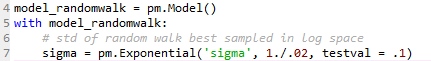
\includegraphics[scale=0.7]{bayesian_random_walk_fix.png}
\end{figure}
\end{frame}

%------------------------------------------------
\begin{frame}
\frametitle{Trouble shooting for package Zipline}
This package seems to be conflicting with python 3.5.0 and above
\begin{figure}[H]
	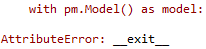
\includegraphics[scale=0.7]{pymc_error_3.png}
\end{figure}
so it is not feasible for us to use zipline, \\
instead we can use pandas just like in the previous section
\end{frame}

%------------------------------------------------
\begin{frame}
\frametitle{Gaussian walk using pandas data}
This is an example of gaussian walk model using pandas library data
\begin{figure}[H]
	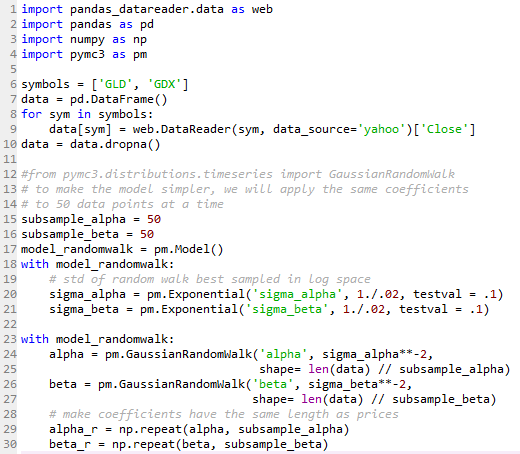
\includegraphics[scale=0.48]{bayesian_gaussian_walk_pandas.png}
\end{figure}
Add pm. in front of GaussianRandomWalk
\end{frame}

%------------------------------------------------
\begin{frame}
\frametitle{Uniform model - errorneous}
There is error occurred when we try to multiply two vectors with different lengths.
\begin{figure}[H]
	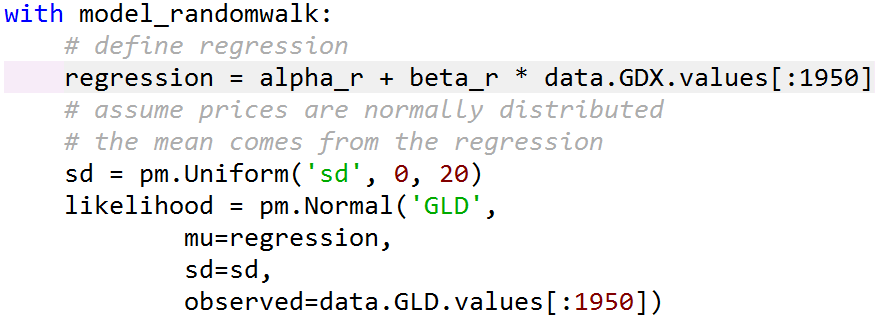
\includegraphics[scale=0.48]{bayesian_error.png}
\end{figure}
This error has not been solved.
\end{frame}

%------------------------------------------------
\begin{frame}
\frametitle{Bayesian regression - optimization}
\begin{figure}[H]
	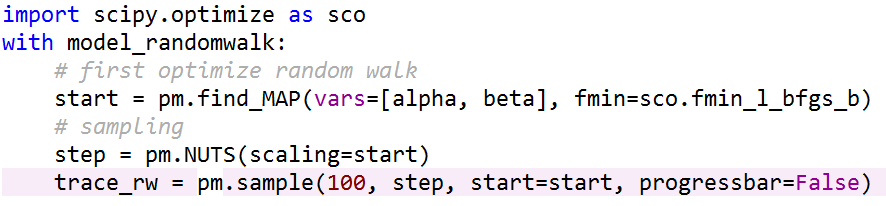
\includegraphics[scale=0.48]{bayesian_optimize.png}
\end{figure}
\end{frame}

\section{Variance Reduction Techniques} %------------------------------------------------

\subsection{Control Variates}

%------------------------------------------------
\begin{frame}
\frametitle{Control Variates - Mathematics}
Our aim is to estimate $\mathrm{E}[Y_{i}]$ \\
Under simulation, we use : $$\bar{Y} = \frac{1}{n} \sum_{i=1}^{n} Y_{i}$$ (unbiased estimate)\\
Now we introduce a new variable $X$, with realizations $X_{i}$, for i from 1 to n\\
Define $Y_{i}(\lambda) = Y_{i} - \lambda (X_{i} - \mathrm{E}(X))$
$$\bar{Y}(\lambda) = \bar{Y} - \lambda (\bar{X} - \mathrm{E}(X)) = \frac{1}{n} \sum_{i=1}^{n} [Y_{i} - \lambda (X_{i} - \mathrm{E}(X))]$$
\end{frame}

%------------------------------------------------
\begin{frame}
\frametitle{Control Variates - Unbiasedness and Consistency}
The new estimate $\bar{Y}(\lambda)$ is unbiased and consistent.\\[5mm]
Unbiasedness: $$\mathrm{E}(\bar{Y}(\lambda)) = \mathrm{E}[\bar{Y} - \lambda(\bar{X} - \mathrm{E}(X))] = \mathrm{E}(\bar{Y}) - \lambda(\mathrm{E}(\bar{X}) - \mathrm{E}(X)) = \mathrm{E}(Y) $$
\begin{equation*}
\begin{split}
Consistency: \lim_{n\to\infty} \frac{1}{n}\sum_{i=1}^{n} Y_{i}(\lambda) 
&=\lim_{n\to\infty} \frac{1}{n}\sum_{i=1}^{n} [Y_{i} - \lambda (X_{i} - \mathrm{E}(X))] \\
&= \mathrm{E}[Y - \lambda(X-\mathrm{E}(X))] \\
&= \mathrm{E}(Y) \\
\end{split}
\end{equation*}
\end{frame}

%------------------------------------------------
\begin{frame}
\frametitle{Control Variates - Controlling Variance of estimate}
\begin{equation*}
\begin{split}
\mathrm{Var}[Y_{i}(\lambda)]
&=\mathrm{Var} [Y_{i} - \lambda(X_{i} - \mathrm{E}(X))] \\
&= \mathrm{Var}[Y_{i} - \lambda X_{i}] \\
&= \mathrm{Var}(Y_{i}) + \lambda^{2}\mathrm{Var}(X_{i}) - 2\lambda\mathrm{Cov}(X_{i}, Y_{i}) \\
&= \sigma_{Y}^{2} + \lambda^{2}\sigma_{X}^{2}-2\lambda\sigma_{X}\sigma_{Y}\rho_{XY}\\
\end{split}
\end{equation*}
\begin{center}
In order to find the minimum variance by varying $\lambda$\\[2mm]
Set $\frac{\partial \mathrm{Var}[Y_{i}(\lambda)]}{\partial \lambda} = 2\lambda \sigma_{X}^{2} - 2\sigma_{X}\sigma_{Y}\rho_{XY}$ to 0:
\end{center}
$$ \lambda^{*} = \frac{2\sigma_{X}\sigma_{Y}\rho_{XY}}{2\sigma_{X}^{2}} = \frac{\sigma_{X}\sigma_{Y}\rho_{XY}}{\sigma_{X}^{2}} = \frac{\mathrm{Cov}(X,Y)}{\mathrm{Var}(X)}$$
\end{frame}

%------------------------------------------------
\begin{frame}
\frametitle{Control Variates - Controlling Variance of estimate}
Compare the new variance with the old:
\begin{equation*}
\begin{split}
\frac{\mathrm{Var} [Y_{i} - \lambda^{*}(X_{i} - \mathrm{E}(X))]}{\mathrm{Var}(Y)}
&=\frac{\sigma_{Y}^{2} + {\lambda^{*}}^{2}\sigma_{X}^{2}-2\lambda^{*}\sigma_{X}\sigma_{Y}\rho_{XY}}{\sigma_{Y}^{2}} \\
&=1+\frac{\frac{\mathrm{Var}(X)(\mathrm{Cov}(X,Y))^{2}}{(\mathrm{Var}(X))^{2}}-\frac{2(\mathrm{Cov}(X,Y))^{2}}{\mathrm{Var}(X)}}{\sigma_{Y}^{2}}\\
&=1+\frac{\frac{\sigma_{X}^{4}\sigma_{Y}^{2}\rho_{XY}^{2}}{\sigma_{X}^{4}}-\frac{2\sigma_{X}^{2}\sigma_{Y}^{2}\rho_{XY}^{2}}{\sigma_{X}^{2}}}{\sigma_{Y}^{2}}\\
&=1+\frac{\sigma_{Y}^{2}\rho_{XY}^{2}-2\sigma_{Y}^{2}\rho_{XY}^{2}}{\sigma_{Y}^{2}}\\
&=1-\rho_{XY}^{2}\\
\end{split}
\end{equation*}
Conclusion from the theoretical results:\\
The stronger the correlation, the better the reduction in variance.
\end{frame}

%------------------------------------------------
\begin{frame}
\frametitle{Choices of Control Variates}
We can use several different random variables as control variates.
\begin{itemize}
	\item Underlying asset prices
	\item Tractable options
	\item Bond prices
	\item Tractable dynamics
\end{itemize}
\end{frame}

%------------------------------------------------
\begin{frame}
\frametitle{Control Variates - Underlying asset prices}
The underlying asset prices provide a source of control variates for its natural correlation with the derivative payoff.\\
The control variate estimator is formed like this:
$$ \frac{1}{n}\sum_{i=1}^{n}(Y_{i}-\lambda[S_{i}(T)-e^{rT}S(0)])$$
For European Call option, $Y = e^{-rT}(S(T)-K)^{+}$.
However, one problem arises: as the strike price goes higher, the correlation of the underlying asset prices and the payoff decreases, this diminishes the effect of control variates upon variance reduction.
\end{frame}

%-----------------------------------------------
\begin{frame}
\Huge{\centerline{Thank You}}
\begin{center}
\begin{normalsize}
\emph{E0007424@u.nus.edu}
\end{normalsize}
\end{center}
\end{frame}

%------------------------------------------------

\end{document} 